\documentclass{book}

%\usepackage{times}
\usepackage[DRAFT]{cslipubs}
%\usepackage{url}
\usepackage{graphicx}
%\usepackage{graphics}
%\usepackage[bookmarks=true, pdfstartview=FitV, colorlinks=true,
%            linkcolor=blue, citecolor=blue, urlcolor=blue]{hyperref}

\usepackage[comma]{natbib}  % CSLI Pubs favored bibliography package.

\usepackage{chapterbib}

\begin{document}

%\conferenceinfo{Second Conference on Online Deliberation / DIAC 2005}{Stanford, CA, USA}
%\setpagenumber{50}
%\CopyrightYear{2005} 
%\crdata{0-12345-67-8/90/01}  \% Allows default copyright data (X-XXXXX-XX-X/XX/XX) 

\title{book name}
\author{editor names}



%\numberofauthors{2}

%\alignauthor Dana~B. Dahlstrom\\
%       \affaddr{Computer Science and Engineering}\\
%       \affaddr{University of California, San Diego}\\
%       \affaddr{9500 Gilman Dr 0114}\\ 
%       \affaddr{La Jolla, CA 92093-0114}\\
%       \email{dana at cs.ucsd.edu}
%\alignauthor Bayle Shanks\\
%       \affaddr{Computational Neurobiology}\\
%       \affaddr{University of California, San Diego}\\
%       \affaddr{9500 Gilman Dr 0346}\\
%       \affaddr{La Jolla, CA 92093-0346}\\
%       \email{bshanks at ucsd.edu}
%}

\date{May 1, 2005}

\maketitle
\achapter{Software support for face-to-face parliamentary procedure}{ Dana B. Dahlstrom and Bayle Shanks}

%\begin{abstract}
\section*{Abstract}
Parliamentary procedure of the sort codified in \emph{Robert's Rules of Order}
is a widely used system of rules for group decision making.
Unfortunately, in many settings where parliamentary procedure is used,
unfamiliarity with the rules inhibits participation,
working against the aim of giving due consideration to each member's opinion. 

This paper describes software that
supports face-to-face parliamentary procedure
by publicly displaying information about items under consideration
and about actions available under the rules.
These features facilitate shared context among the participants,
encourage adherence to the rules, and
help novices engage and learn the process.
% Motivations and principles for the project are given
% and related to previous work,
% preliminary results are reported, and
% future work is proposed.
%\end{abstract}

\section{Introduction}  % 0.5

% Parliamentary procedure of the sort codified in Robert's Rules of Order
% is a widely used system of rules for group decision making.

Parliamentary procedure is a centuries-old, evolving tradition of rules and customs for group decision making. It aims for full and free discussion, safeguarding the rights of the minority and of individual members, even in the face of intense disagreement. The houses of UK Parliament and of the US Congress, for example, each have their own parliamentary rules; but the best-known codification is called \emph{Robert's Rules of Order}, after Henry Robert, who wrote the first popular manual on parliamentary law in the late-19th-century United States.

Parliamentary procedure is used in many different organizations ranging from small boards and committees to governmental legislative bodies. A group meeting using Robert's Rules of Order is called a \emph{deliberative assembly} and requires that all members communicate synchronously by voice, normally face-to-face. A deliberative assembly may have from a few to a few hundred members.

% \citealt{robert:rules}
Central to Robert's Rules of Order are \emph{motions}, by which a member may propose that the assembly take certain actions. The ``Table of Rules Relating to Motions'' in the 1915 version of \textit{Robert's Rules of Order Revised}, now in the public domain, includes 45 different motions that fall mostly into 4 classes: main motions, subsidiary motions, incidental motions, and privileged motions. \emph{Precedence} among and within the classes specifies which motions are \emph{in order}---that is, permitted by the rules---depending on which motions are currently pending.

Each class of motions has general characteristics, and many individual motions have peculiarities of their own. Some motions are debatable; others are not; some are amendable; some allow subsidiary motions applied to them; some can be reconsidered. Most require first obtaining the floor, being seconded, and a majority vote in the affirmative to be adopted; others may interrupt a speaker, need not be seconded, and require no vote; yet others require a two-thirds vote. In short the rules are many and difficult to remember, especially in a lively meeting.

\subsection{Procedural Difficulties}

% Unfortunately, in many settings where parliamentary procedure is used,
% unfamiliarity with the rules inhibits participation,
% working against the aim of giving due consideration to each member's opinion.

The complexity of parliamentary procedure can be challenging for anyone, and particularly stifling to a novice participant who knows little or nothing of the rules. He or she may have opinions to voice or objectives to accomplish, but not know how. Robert's Rules of Order allow a \emph{parliamentary inquiry} by which a member may ask for advice on such matters, but the member must know this option is available and the chair must be prepared to give an appropriate response.

% Unwitting deviation from the rules can impinge on fundamental rights.

In many organizations that nominally use parliamentary procedure, even the chair of an assembly is only vaguely familiar with the rules, often having learned mainly from experience in meetings and never having studied a manual. One problem that can arise in such circumstances is that the assembly may take action without due process, and in doing so violate fundamental rights of the minority, of individual members, or of the assembly itself.

For example, one common misbelief about parliamentary procedure is that any member may halt debate and initiate a vote at any time by shouting, ``I call the question!'' In fact, to ``call the question'' or, more properly, to move the \emph{previous question}, one must obtain the floor in order to make the motion, and it must be seconded and finally itself receive a two-thirds vote in the affirmative. Robert's Rules of Order consistently emphasize that suppressing debate requires the support of two thirds; this requirement protects the fundamental right to have questions thoroughly discussed before taking action. Absent knowledge of the rules, this fundamental right is easily violated.

% Participants who misunderstand or lose track of the proceedings
% miss important opportunities to give input.

% participants can lose track of process/state
%   especially in large meetings with (useful) side-discussions
%   anecdote from UCSA congress

Even when members have a working knowledge of the rules and their fundamental rights are intact, participants can lose track of the proceedings for a variety of reasons. Parliamentary procedure is formally linear and verbal and relies on shared context. 
When one loses context in a deliberative assembly, one may rise to a \emph{point of information} in order to ask questions, but this may be socially awkward. If participants miss something, it is easy to become confused about what has happened or what is happening.


\subsection{Our software}
\label{sec:support-technology}

% software to support group deliberation using parliamentary procedure

% This paper describes software that
% supports face-to-face parliamentary procedure
% by publicly displaying information about items under consideration
% and about actions available under the rules.

% These features facilitate shared context among the participants,
% encourage adherence to the rules, and
% help novices engage and learn the process.

% run on common portable computers
%   ideally connected to display large enough for group
% support novice participants
%   indicate available/relevant motions
% aid rule enforcement

This paper describes software that can run on a portable computer connected to a digital projector. A single user enters events as they transpire, such as motions and votes. Based on this input, the software keeps track of the meeting state and updates the large display so that at any time, assembly members can see information such as currently pending motions, motions currently in order, and transacted business.


The prototype application shown in Figure \ref{fig:user-interface} is operated in a face-to-face meeting conducted according to Robert's Rules of Order. It is written using the Parliament module (\citealt{shanks2006}), and is freely available.\footnote{http://parliament.sourceforge.net/} 

% \footnote{\url{http://parliament.sourceforge.net/}} 
 

% !!! "and characteristics"

% !!! applicable rules: requires second? debatable? vote required?
% procedural reminders such as when a motion requires a second, whether it is debatable, what vote needed for its adoption

\section{Design Considerations}  % 3

A main concern is which information to display in the interface, especially as there are too many motions to display at once.

% who does the work, who gets the benefit [ref: Grudin]
\label{sec:secretary} A second design goal is to serve the secretary's needs. Under Robert's Rules of Order, the duties of the secretary include several activities: preparing of an order of business for the chair; tending business that is postponed, laid on the table, or left unfinished; and producing the minutes. The system is intended in part to aid the secretary in executing these duties.

Assisting the secretary is not merely ancillary. As \citealt{grudin:groupware} has pointed out, the disparity between who does the work and who gets the benefit is often a barrier to acceptance of groupware systems. While it aims to benefit many individuals and the group as a whole, this system requires someone to do work: continually and promptly entering meeting proceedings into a computer. Helping get the secretary's job done is a key incentive for this work.

\label{sec:live-setting}

A third requirement for the interface is that it be quick and flexible enough to keep up with live action. The user must not get backlogged entering events; a public display of obsolete information is worse than useless.

Finally, the interface must gracefully handle at least two kinds of irregularities: mistakes by the user, which must be promptly correctable; and deviations from the ordinary rules, either by a motion to \emph{suspend the rules} or by mistake.




\subsection{Use Considerations}  % 3
\label{sec:caveats}

% it must be clearly established that the chair, not the software, is
%   authoritative


% to prevent confusion, the chair should monitor the software display and
%   instruct the operator to correct it when necessary

When software support for parliamentary procedure is introduced, it should be made clear that the chair, not the software, presides over the assembly. 
However, to prevent confusion, it is crucial for the chair to monitor the output of the software to ensure the information being recorded and displayed to the assembly is correct.
   

The software should not be considered a parliamentary authority or a substitute for knowledge of the rules. One of the chair's responsibilities is to advise members on how to achieve their aims; in most cases, simply ruling a motion out of order will not do. Because Robert's Rules of Order are intricate and rely on subjective determinations, the software's capacity to settle parliamentary questions is necessarily limited. The chair should be familiar with the rules and have a copy of the assembly's parliamentary authority at the meeting.


%   all this being said, certain socially awkward tasks such as floor control
%     and enforcing time limits could be more accurately and impartially

Computers are oblivious to social conventions, which makes them less fit for many tasks of chairmanship, but perhaps more fit for others. For example, enforcing time limits can be socially awkward, but is often generally appreciated so long as it is done fairly.

% \section{Implementation} 
% \label{sec:implementation}

% prototype system built on and co-developed with Parliament
%   software module for rule-based
%     (collaboration|communication|interaction|deliberation)
%     written in Python [ref]
%   beyond the module itself, our "meeting helper" prototype comprises
%     a working specification of Robert's Rules of Order, and
%     an interface written using PythonCard [ref]

% \footnote{\emph{Parliament} is an open-source software module that implements the logic and bookkeeping functions necessary for the function of parliamentary procedure.}

\section{The User Interface}

Figure~\ref{fig:user-interface} depicts the user interface, designed for a single user such as an organization's secretary. The window which is displayed on the projector is different.

The \emph{motions currently in order} contains a list of only those motions that are in order at the present time. The user may activate any of these motions to indicate that that motion has been moved in the meeting. There are text fields for the number of affirmative and negative votes and a button to compare the tallies to the proportion of votes required by the rules. \emph{Adopted} and \emph{rejected} buttons allow the user to indicate the fate of the immediately pending motion directly when votes are not counted. \emph{Back} and \emph{forward} buttons navigate through meeting history, providing a multiple undo/redo mechanism.

The \emph{currently pending motions} in the tree diagram can be selected, populating several other fields with information about the selected motion. In addition to the \emph{text} of the motion, these also include its \emph{mover} and its \emph{target}. All of these fields are editable by the user.

The interface also provides an \emph{event log} with a record of each motion, and whether that motion was adopted or rejected.

Real-world assemblies sometimes deviate from the rules. To be useful, the software must continue to track the state of the meeting. Hence the interface provides an \emph{ignore rules} checkbox that allows the user to record actions and motions despite these being out of order according to the module's interpretation of the rules.


\begin{figure*}
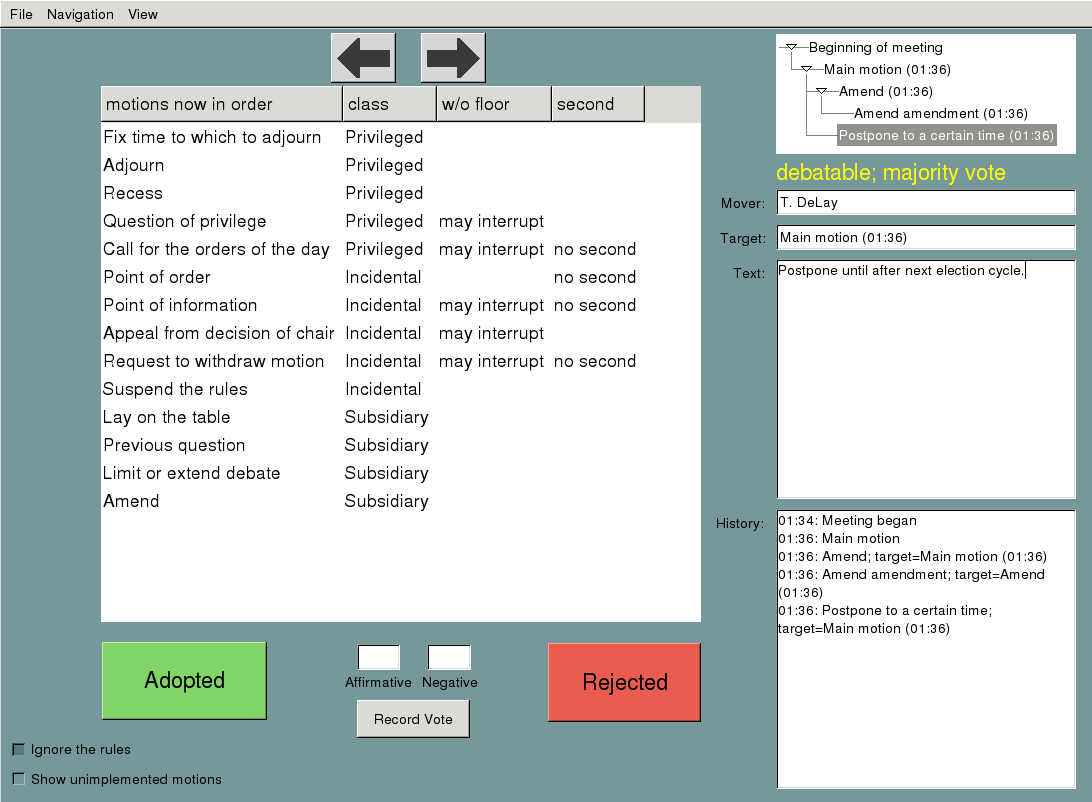
\includegraphics[scale=.7]{user}
%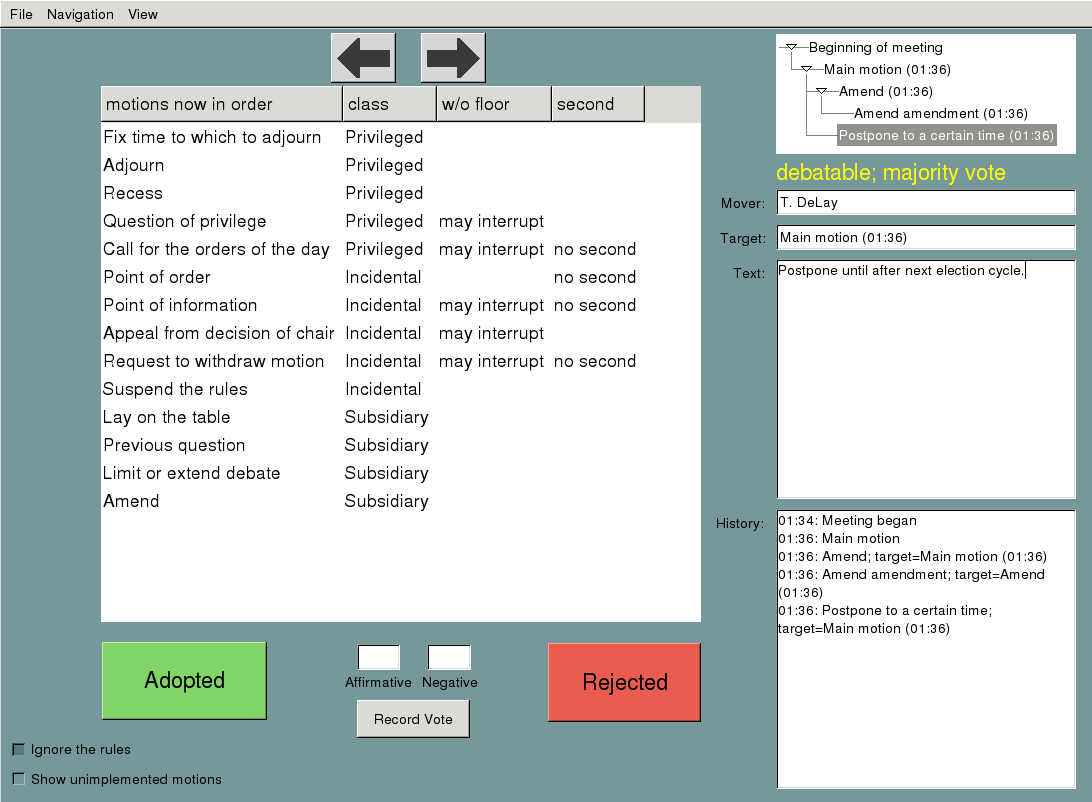
\includegraphics{user}
\caption{The user interface.}
\label{fig:user-interface}
\end{figure*}
 
\section{Results of Preliminary Trials}  % .75

% preliminary experience
%   used at one meeting of GSAUCSD
%   lessons learned

The prototype has been pilot-tested in meetings of the Graduate Student Association Council at UCSD. 

One problem was the physical arrangement of the room. Since members spend much of the meeting looking toward the chair, who faces them, it seemed fitting to place the projected display behind the chair. However, this meant the chair could not see the display. That made it difficult for the chair to realize when the software was displaying inaccurate information.

A projector screen displaying inaccurate information about the state of the meeting is potentially disastrous and should be avoided. Meeting participants may rely on the projected information which, if inaccurate, will hinder rather than help. Therefore, the chair should keep aware of what the software is displaying and see that it is corrected when necessary.

One solution is for the system's operator (perhaps the secretary) to sit next to the chair. This way, though the projected display may not be visible to the chair, the computer screen will be. 

Preliminary experience confirms that when a computer and projector are introduced into a meeting, people want to put the equipment to various uses. Members of GSAUCSD asked us to launch other software on the computer in order to display their governing documents and long resolutions under consideration.


\section{Relation to Other Work}  % .5

There is a considerable body of work on electronic meeting systems and systems to support group decision making, whether face-to-face or otherwise, but little work has focused on parliamentary procedure.

%\subsection{Group Decision Support Systems}

% idea specifically proposed by DeSanctis & Gallupe [ref]
%   classified in Level 3 (describe)

A \emph{group decision support system (GDSS)} employs technology to facilitate group decision making. A GDSS is \emph{groupware}, in that it is designed for multiple people working collaboratively. As a field, GDSSs are related to \emph{decision support systems (DSS)}, although the latter typically focus on information gathering and analysis for a single individual.

A GDSS to apply parliamentary procedure was envisioned at least as early as 1987 by DeSanctis and Gallupe. In their nomenclature, such a system is called a \emph{Level 3 GDSS}. While Level 1 GDSSs aim only to facilitate communication and Level 2 GDSSs passively offer tools and models, Level 3 GDSSs actively apply rules regulating the decision process.

%   system described here also uses elements of L1, but not L2

\citealt{kraemer:computer-based}, in their survey of systems for cooperative work and group decision support, argue that ``most of the efforts to apply these technologies have affected decision processes too much or too little to provide a good assessment of their effects.'' On one hand, audiovisual presentation and teleconferencing technologies merely speed up process without improving the quality of decision making; on the other hand, technology that imposes structured collaboration techniques also imposes the designers' views of the decision process on the participants.

% Kraemer and King GDSS taxonomy: decision conference

Our software aims to improve group decision making without externally imposing structure; many organizations have already adopted a parliamentary authority such as Robert's Rules of Order. 

A number of GDSSs have been built. For example, \citealt{davies:online} have built an online deliberation environment, \emph{Deme}, primarily to supplement the activities of groups that already meet face-to-face.

% D&G ``Robert's rules of order, or discussion procedures self-designed by the group''
% D&G ``Legislative Session ... meeting proceedings can be recorded''
% D&G ``Computer-Mediated Conference ... large, dispersed groups responsible for decisions''
% D&G ``users must have extended experience with GDSS before the effectiveness or ineffectiveness of systems design can be fully assessed.''
% D&G ``Performance/Satisfaction Tradeoff ... high quality decisions, or a high sense of satisfaction ... improve the efficiency and effectiveness of group decision making

% original motivation for Parliament: online deliberation
%   "Doug Schuler proposed in his 1996 book New Community Networks that
%    Roberts Rules of Order could be used as a basis for online deliberation."

% face-to-face meetings have useful properties
%   simultaneous shared attention, intersubjectivity
%     rich communication channel, quick exchange, synchronizing
%   live meetings complement online collaboration
% integrate in-person with online deliberation

% \subsection{EMS papers}
% 
% Nunamaker \textit{et al.} \citealt{nunamaker:electronic}
% 
% Hayne \citealt{hayne:facilitators}

\subsection{Work Related to Robert's Rules of Order}

Some aspects of parliamentary procedure are oriented toward a face-to-face setting, but the underlying principles and many of the rules can be applied to decision-making groups using various other modes of communication.

\citealt{zhang:rule-mitigated} designed a document-based collaboration system based on an ``agenda item life cycle'' inspired by Robert's Rules of Order.

% \citealt{chang:rule-mitigated,zhang:rule-mitigated}. 

\citealt{horan:protocol} describe a protocol for conducting deliberations by e-mail in academic committees using Robert's Rules of Order. 

\emph{Robert's Rules in Motion}\footnote{http://imovethat.com/} is a commercially available single-user application that simulates meetings in order to train the user in the use of parliamentary procedure.

% \url{http://imovethat.com/}

% Chang \textit{et al.} \citealt{chang:rule-mitigated}
% 
% not really the rules of parliamentary procedure
%   but a simple "agenda item life cycle" inspired by RRO proceedings
% extended RRO for electronic collaboration
%   eliminate unique floor, allow concurrency
%     discussion threads
%   limit on nesting of amendments is unnecessary
%   abolition of motion to recess
%   electronic meeting may be adjourned only once, when the work is concluded
%   provide a mechanism for modifying the agenda
%   motions to modify assembly membership

% \subsection{OD papers}

% Davies \textit{et al.} \citealt{davies:community}

% Witschge \citealt{witschge:online}

% Davies \textit{et al.} have built an online deliberation environment, \emph{Deme} \citealt{davies:online}, primarily to supplement the activities of groups that already meet face-to-face.

% \subsection{OD projects}

% Robert's Rules Assembly\footnote{\url{http://grace.evergreen.edu/~powmat25/RR/Home.html}}

% e-Liberate\footnote{\url{http://trout.cpsr.org/program/sphere/e-liberate/about.php}}

% Public Sphere Project\footnote{\url{http://trout.cpsr.org/program/sphere/}}

% Deme\footnote{\url{http://groupspace.org/}}

% \subsection{Other projects}

% GroupSystems\footnote{\url{http://www.groupsystems.com/}}

% ActionForum.com\footnote{\url{http://www.actionforum.com/}}

% Facilitate.com\footnote{\url{http://facilitate.com/}}


\section{Conclusions}  % .25

The technology described herein shows promise for improving the practice of parliamentary procedure in face-to-face meetings. Assemblies with members not well practiced in the rules can especially benefit from such a system.


Software support for parliamentary procedure fills a unique niche among similar research. By supporting group work while having a single user operating the interface, it avoids many pitfalls of groupware applications. By aiming to improve group decision making without externally imposing structure, parliamentary-procedure software offers opportunities to study effects on groups that were obscured by the more dramatic interventions of other group decision support systems.

Parliamentary-procedure software should run on common portable computers, and be easy for any organization's secretary to learn and use, streamlined enough to keep pace with live meetings, and flexible enough to handle the adaptive circumvention of rules that inevitably occurs in real assemblies. The software should generate a record from which official minutes can be produced, and which may in the future be a medium for interoperation with online deliberation systems.

Preliminary experience with a prototype system in real meetings has met with enthusiastic response. Further development and experimentation is underway.

\bibliographystyle{cslipubs-natbib}  % 1.0
\bibliography{parliprosoft}
 
\end{document}
